%Please use LuaLaTeX or XeLaTeX
\documentclass[11pt,aspectratio=169]{beamer}
\usepackage{amsmath}
\usepackage{amssymb}
\usepackage{amsfonts}
\usepackage{mathrsfs}
\usepackage[font=scriptsize]{caption}
\usepackage{bm}
\usepackage[
    backend=biber,
    style=authoryear,
    sorting=nyt
]{biblatex}
\addbibresource{../doc/references.bib}
\DeclareMathOperator{\sgn}{sgn}

\title{Introducing PlesioGeostroPy \\ {\normalsize a Python realization of the PG model}}
\date[Oct 2023]{Oct. 2023}
\author{Min, Jingtao}
\institute{EPM Group, Institut für Geophyik, ETH Zürich}

\usetheme{eth}

\colorlet{titlefgcolor}{ETHBlue}
\colorlet{accentcolor}{ETHRed}

\begin{document}

%\def\titlefigure{elements/title-page-image}		% Default image
%\def\titlefigure{elements/title-page-image-43}	% Use this for 4:3 presentations

\colorlet{titlefgcolor}{ETHPurple}
\setlength{\titleboxwidth}{0.6\textwidth}			% Change box width
\titleframe

% \colorlet{titlefgcolor}{ETHPurple}
% \def\titlefigure{elements/title-page-image-alt}
% \title{Different background}
% \titleframe

% \colorlet{titlebgcolor}{ETHGreen}
% \def\titlefigure{}
% \setlength{\titleboxwidth}{0.75\textwidth}			% Change box width
% \title{Or even a plain color, especially if your title is very long and leaves no space for what's behind the colored box}
% \titleframe

% \tocframe

\section{The PG model}
\begin{frame}{PG, QG, and all the geostrophic models}
    
\end{frame}

\begin{frame}{How did I end up here?}
    Since the start of my doctoral studies, I
    \begin{itemize}
        \item studied surface operators and tried to derive the boundary terms in the diffusive torsional oscillation (TO) equation for \textcolor{blue}{2 months} $\Longrightarrow$ didn't lead anywhere;
        \item studied torsional Alfvén waves and calculated the 1-D eigenmodes of the torsional oscillation for \textcolor{blue}{2 month} $\Longrightarrow$ didn't lead anywhere;
        \item studied anelastic approximation for \textcolor{blue}{1 month} in order to work on the anelastic version of QuICC, which may help the Jupiter simulation $\Longrightarrow$ project was called off and deemed unpromising before I could start to think about the numerics;
        \item picked up the thread and studied the reflection of Alfvén waves at the fluid-solid interface for \textcolor{blue}{2 months} $\Longrightarrow$ wrote a sixty-page document and yet had more questions than before;
        \item have been mainly working on the PG model since Aug 2023.
    \end{itemize}
\end{frame}

\section{The old implementation}
\begin{frame}{The old implementation - code \textit{Daria}}
    Mathematica implementation (previous member of the group, Dr. Daria Holdenried-Chernoff)
    \begin{figure}
        \centering
        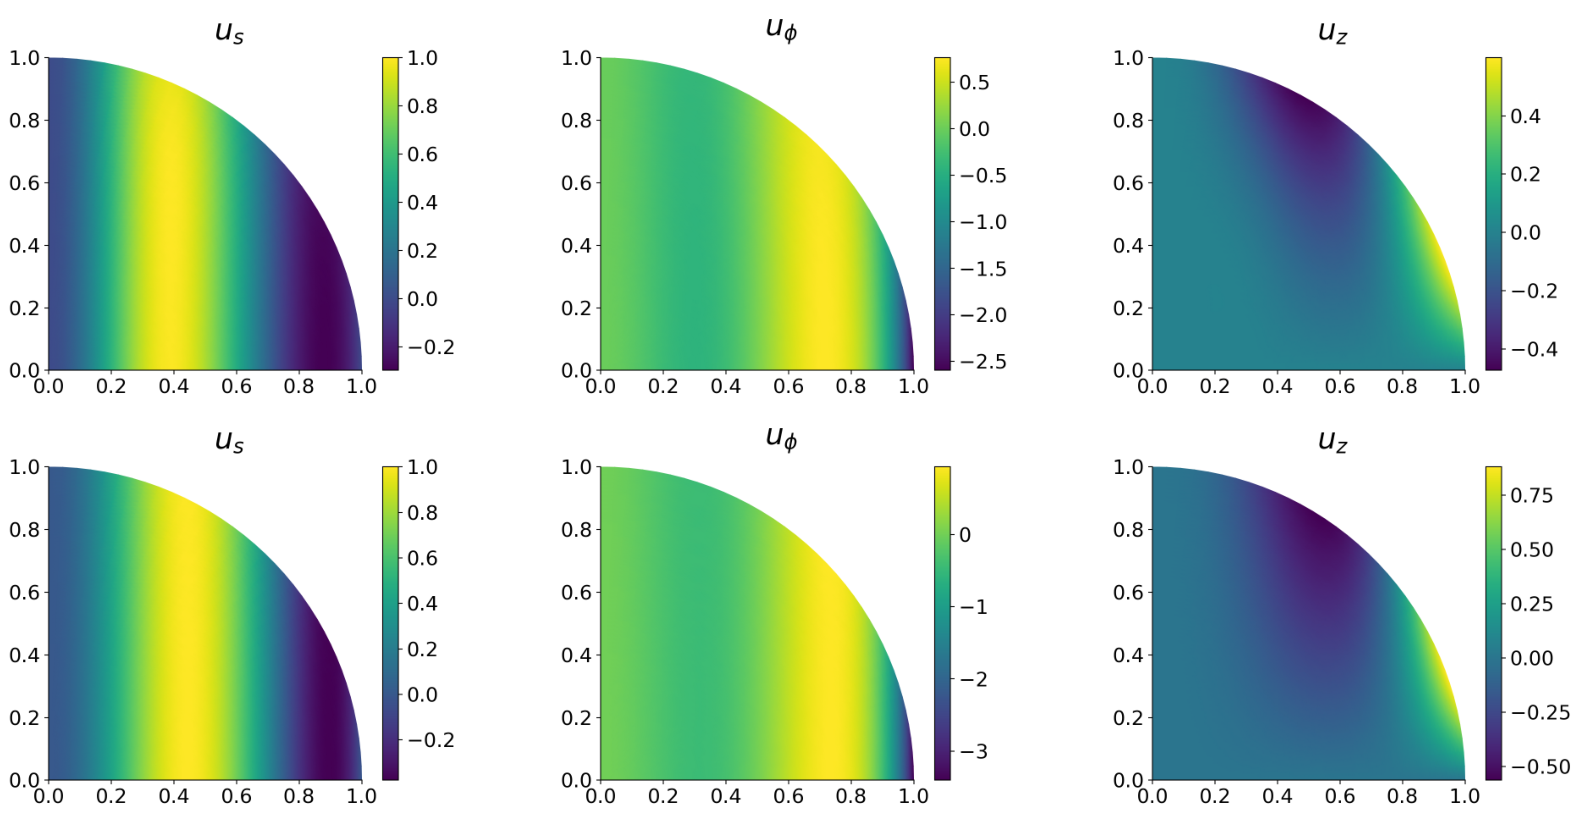
\includegraphics[width=.6\linewidth]{elements/Daria__toroidal_bg_eigen1033-922.png}
        \caption{Eigenmodes calculated using 3-D code \textit{Jiawen} (top) and PG code \textit{Daria}.}
    \end{figure}
    \textcolor{red}{Why reinvent the wheels when we already have a functioning implementation?}
\end{frame}

\begin{frame}{The old implementation - code \textit{Daria}}
    Citizens of Gotham, riddle me this... what is this code snippet doing?
    \begin{figure}
        \centering
        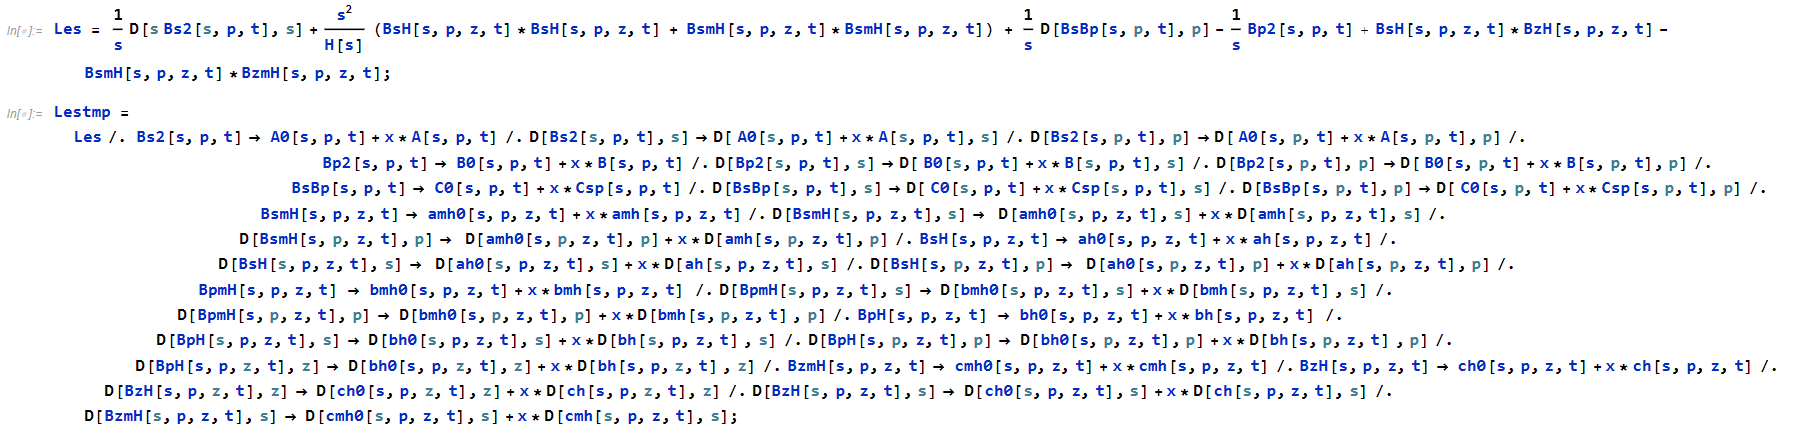
\includegraphics[width=\linewidth]{elements/Mathematica_snippet_1.png}
    \end{figure}
	\pause
	This rewrites the magnetic quantities in Lorentz force $\overline{L_\phi}$ as background + perturbation for linearization.

	e.g. \texttt{Bp2[s, p, t]->B0[s, p, t] + x*B[s, p, t]} equals to $\overline{B_\phi^2} = \overline{B_\phi^2}_0 + \epsilon \overline{B_\phi^2}'$
\end{frame}

\begin{frame}{The old implementation - code \textit{Daria}}
	\begin{columns}
	\begin{column}{.6\linewidth}
		\begin{figure}
			\centering
			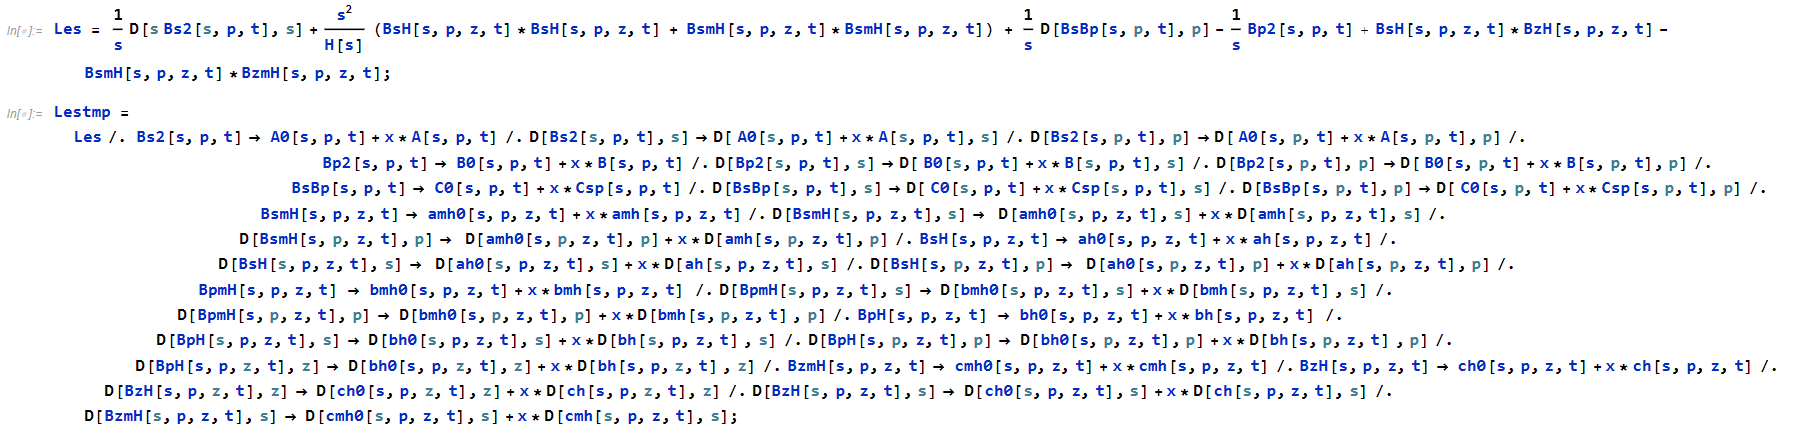
\includegraphics[width=\linewidth]{elements/Mathematica_snippet_1.png}
		\end{figure}
		Why is the code undesirable for \textcolor{red}{developers} and \textcolor{blue}{users} alike?
		\begin{itemize}
			\item long, repetitive operations $\Longrightarrow$ hard to \textcolor{red}{debug}
			\item namings: the background and perturbation fields are named from \texttt{A} to \texttt{H} $\Longrightarrow$ hard to \textcolor{red}{debug} or \textcolor{blue}{invoke}.
			\item At some point I even need a correspondence table to decipher the code.
		\end{itemize}
	\end{column}
	\pause
	\begin{column}{.4\linewidth}
		\begin{figure}
			\centering
			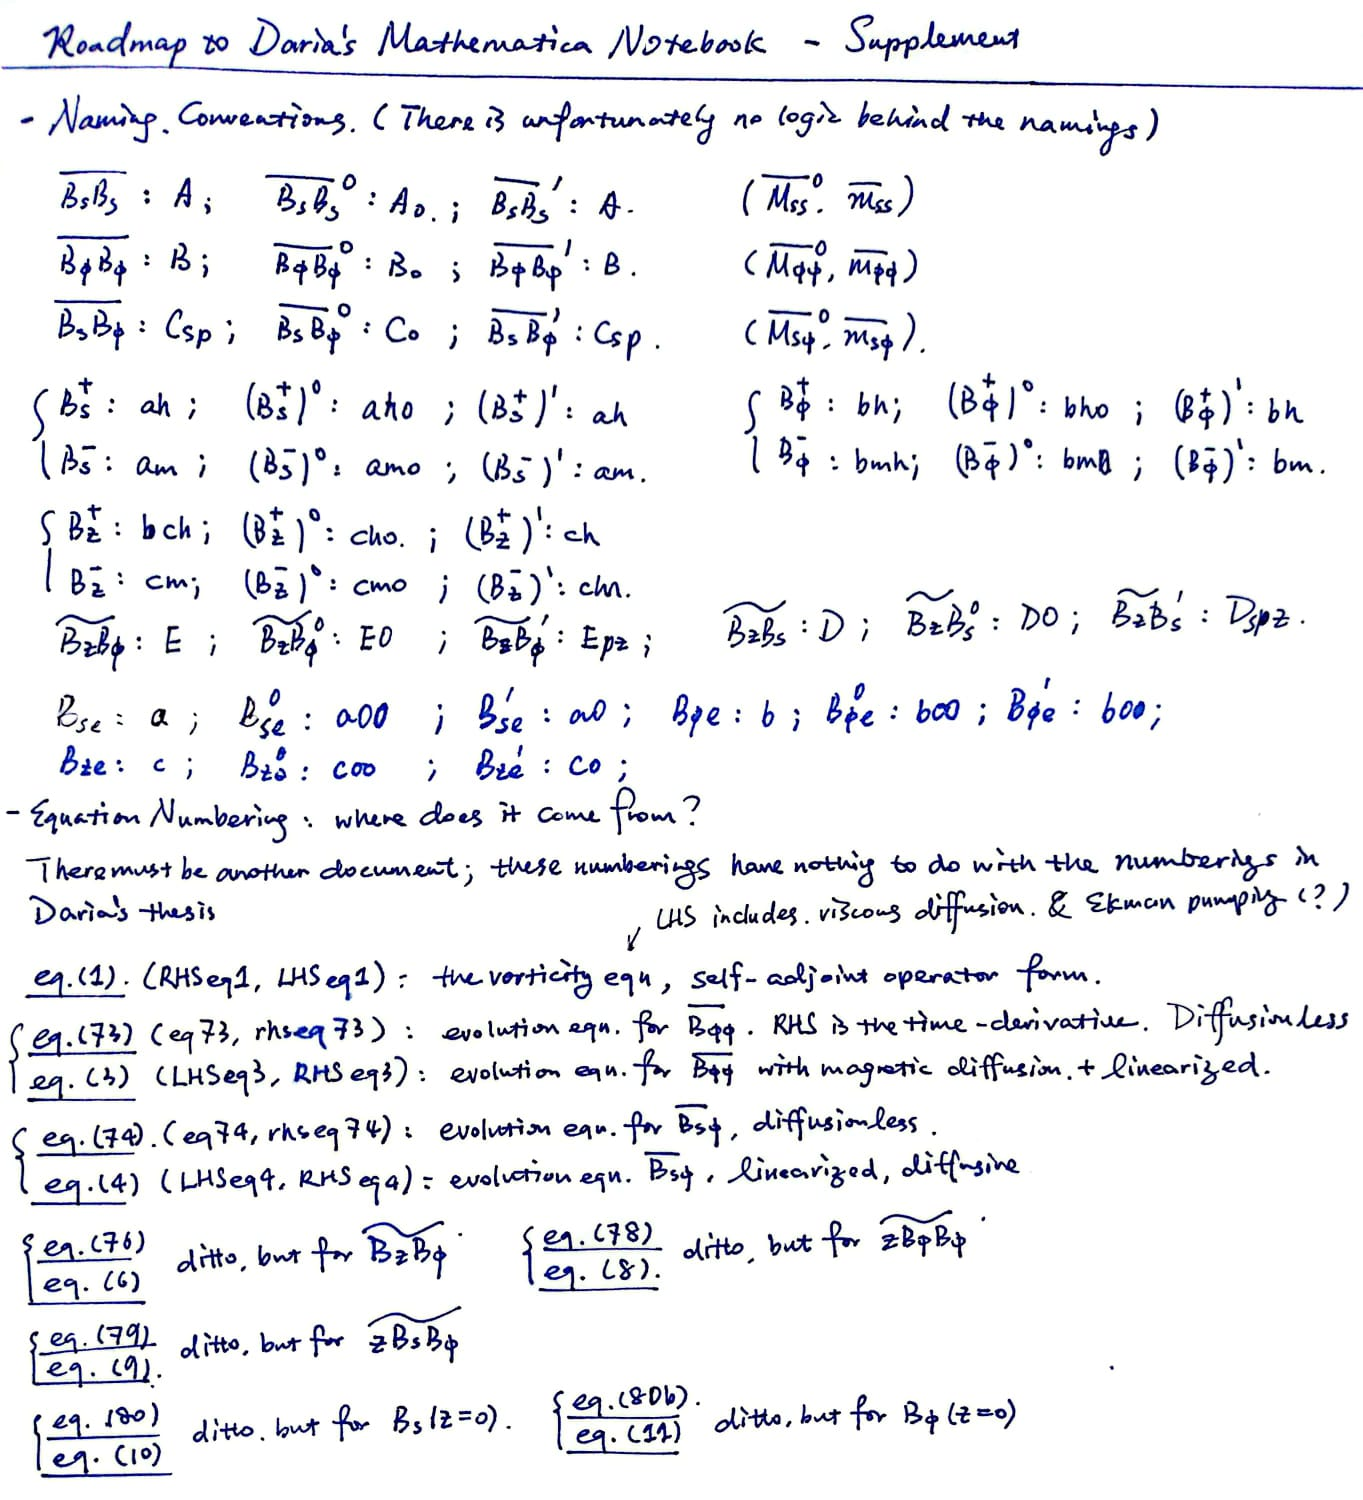
\includegraphics[width=.9\linewidth]{elements/correspondence_table.jpeg}
			\caption{List of physical variables and their names in the code.}
		\end{figure}
	\end{column}
	\end{columns}
\end{frame}

\begin{frame}{The old implementation - code \textit{Daria}}
\begin{columns}
\begin{column}{.46\linewidth}
    \begin{figure}
        \centering
        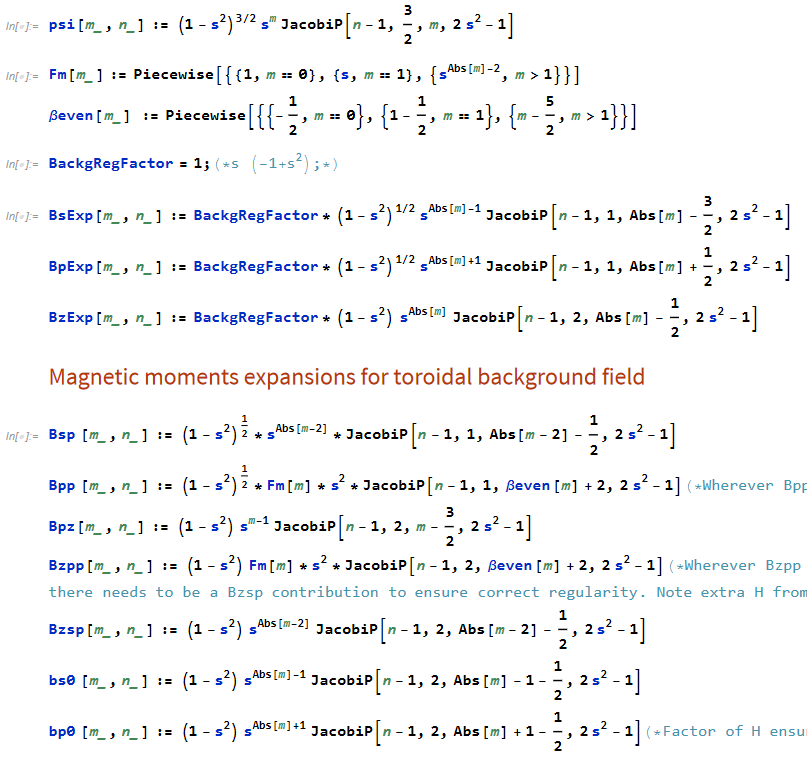
\includegraphics[width=\linewidth]{elements/Mathematica_snippet_expansion.png}
    \end{figure}
\end{column}
\begin{column}{.46\linewidth}
	Inflexible expansions: the expansion and the construction of matrices are hard coded in each notebook.
	\vspace{1em}

	To change the expansion, one needs to 
	\begin{itemize}
		\item produce a complete new Mathematica notebook;
		\item manually change the way the code collects the matrix elements.
	\end{itemize}
	\vspace{1em}

	Especially cumbersome to implement coupling, or if the bases do not coincide with the field quantities (more detail later).
\end{column}
\end{columns}
\end{frame}

\begin{frame}{The old implementation}
	\begin{columns}
	\begin{column}{.46\linewidth}
		Other problems
		\begin{itemize}
			\item The code is not efficient numerically, nor easily linked to efficient numerical libraries.
			\item Cryptic Mathematica syntax sugars
		\end{itemize}
		\begin{figure}
			\centering
			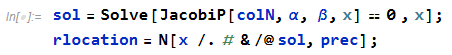
\includegraphics[width=.8\linewidth]{elements/Mathematica_snippet_3.png}
		\end{figure}
	\end{column}
	\begin{column}{.46\linewidth}
	\end{column}
	\end{columns}
\end{frame}

\section{Introducing PlesioGeostroPy}
\begin{frame}
    
\end{frame}

\section{Future works}

\begin{frame}{Regularity conditions for vectors}
	Vector $\mathbf{A} = A_s \hat{\mathbf{s}} + A_\phi \hat{\bm{\phi}} = A_x \hat{\mathbf{x}} + A_y \hat{\mathbf{y}}$

	$A_s$ and $A_\phi$ being regular functions of $s$ and $\phi$ is not sufficient for $\mathbf{A}$ to be regular.
	\vspace{1em}

	E.g. $A_s = A_\phi \equiv 1 \quad \Longrightarrow \quad A_x = \cos\phi - \sin\phi = \frac{x - y}{\sqrt{x^2 + y^2}},\quad A_y = \cos\phi + \sin\phi = \frac{x + y}{\sqrt{x^2 + y^2}}$

	\begin{figure}
		\centering
		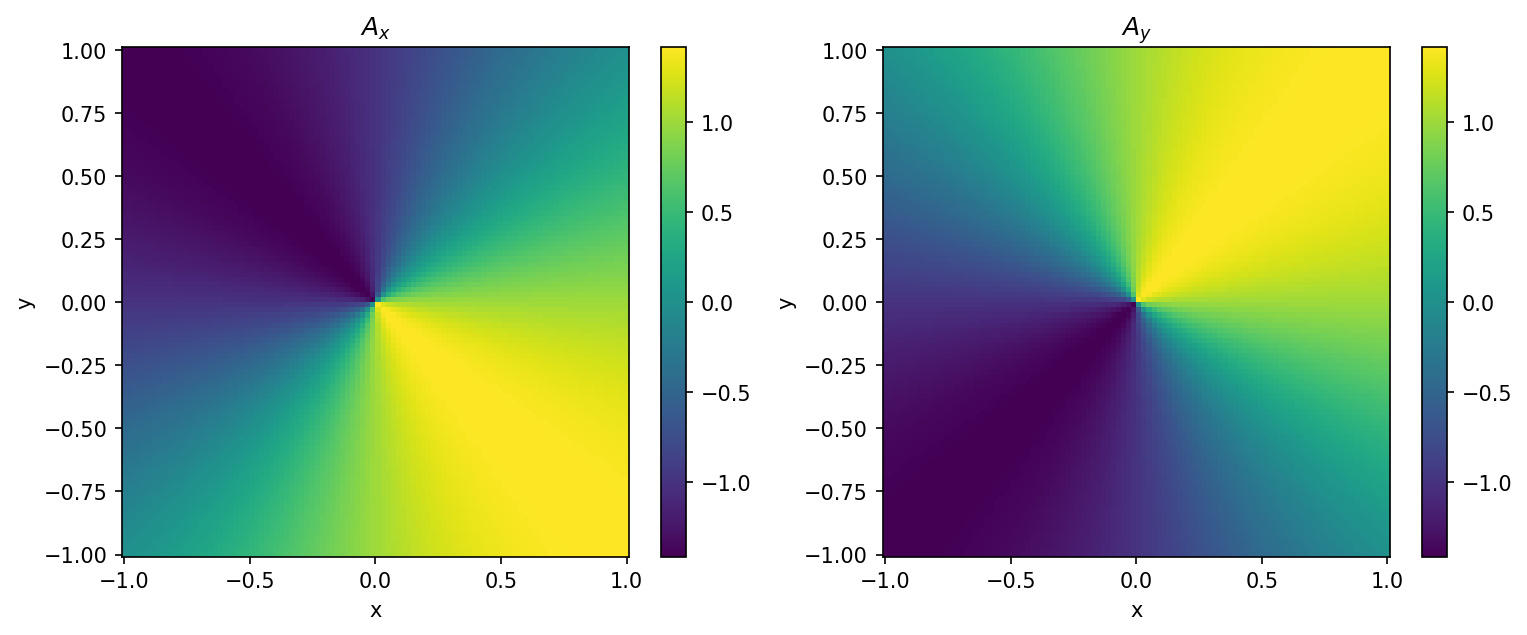
\includegraphics[width=.75\linewidth]{./elements/singular_field.png}
	\end{figure}
\end{frame}

\begin{frame}{Regularity conditions for vectors}
	However, $A_x$ and $A_y$ being regular functions of $x$ and $y$ \textbf{is sufficient} for $\mathbf{A}$ to be regular.
	\textcite{lewis_physical_1990} derived the regularity conditions on Fourier coefficients
	\begin{itemize}
		\item Expand $A_s$ and $A_\phi$ in Fourier series;
		\item Convert to vector components in Cartesian coordinates, 
		\[
			\begin{pmatrix} A_x \\ A_y \end{pmatrix} = 
			\begin{pmatrix} \cos\phi & -\sin\phi \\ \sin\phi & \cos\phi \end{pmatrix} 
			\begin{pmatrix} A_s \\ A_\phi \end{pmatrix}
		\]
		and derive Fourier expansion of $A_x$ and $A_y$.
		\item Replace
		\[
			e^{i|m|\phi} = \frac{(x + iy)^{|m|}}{s^{|m|}},\quad e^{i|m|\phi} = \frac{(x - iy)^{|m|}}{s^{|m|}}
		\] 
		\item $A_x$ and $A_y$ are regular if the resulting rational terms are regular.
		\end{itemize}
\end{frame}

\begin{frame}{Regularity conditions for vectors}
	The required ansätze for vectors in polar coordinates
	\[\begin{aligned}
		A_s &= s g_0 + \sum_{m\neq 0} \left(\lambda_m s^{|m|-1} + g_m s^{|m|+1}\right) e^{im\phi}, \\ 
		A_\phi &= s h_0 + \sum_{m\neq 0} \left(i \sgn(m) \lambda_m s^{|m|-1} + h_m s^{|m|+1}\right) e^{im\phi},
	\end{aligned}\]
	where $g_m = g_m(s^2)$, $h_m = h_m(s^2)$. The Fourier coefficients of $A_s$ and $A_\phi$ are coupled at the lowest order (of Taylor series) in $s$.
\end{frame}

\begin{frame}{Regularity conditions for rank-2 tensors}
	Similar idea, now
	\[
    \begin{pmatrix} A_{xx} & A_{xy} \\ A_{yx} & A_{yy} \end{pmatrix} = 
    \begin{pmatrix} \cos\phi & -\sin\phi \\ \sin\phi & \cos\phi \end{pmatrix}
    \begin{pmatrix} A_{ss} & A_{s\phi} \\ A_{\phi s} & A_{\phi\phi} \end{pmatrix}
    \begin{pmatrix} \cos\phi & \sin\phi \\ -\sin\phi & \cos\phi \end{pmatrix}
	\]
	Proceed similarly as follows
	\begin{itemize}
		\item Expand $A_{ss}$, $A_{s\phi}$, $A_{\phi s}$, $A_{\phi\phi}$ in Fourier series
		\item Convert to components Cartesian coordinates
		\item Rewrite exponentials as polynomials in Cartesian coordinates
		\item $A_{xx}$, $A_{xy}$, $A_{yx}$ and $A_{yy}$ are regular if the resulting rational terms are regular.
	\end{itemize}
\end{frame}

\begin{frame}{Regularity conditions for rank-2 tensors}
	Regularity conditions.
	\[
		\begin{aligned}
			A_{ss}^m + A_{\phi\phi}^m &= s^{|m|} C(s^2) \\ 
			A_{s\phi}^m - A_{\phi s}^m &= s^{|m|} C(s^2) \\ 
			A_{ss}^m - A_{\phi\phi}^m + i \left(A_{s\phi}^m + A_{\phi s}^m\right) &= s^{|m+2|} C(s^2) \\ 
			A_{ss}^m - A_{\phi\phi}^m - i \left(A_{s\phi}^m + A_{\phi s}^m\right) &= s^{|m-2|} C(s^2)
		\end{aligned}
	\]
	Assuming the Fourier coefficients
	\[A_{ij} = \sum_m e^{im\phi} A_{ij}^{m}(s) = \sum_m e^{im\phi} s^{|m|+\Delta_m} \sum_k A_{ij}^{mk} s^{2k}\]
\end{frame}

\begin{frame}{Regularity conditions for rank-2 tensors}
	The required form of the Fourier coefficients
	\[
		\begin{aligned}
			m = 0 :& \quad \left\{\begin{aligned}
				A_{ss}^0 &= A_{ss}^{00} + s^2 C(s^2) \\ 
				A_{\phi\phi}^0 &= A_{\phi\phi}^{00} + s^2 C(s^2) \\ 
				A_{s\phi}^0 &= A_{s\phi}^{00} + s^2 C(s^2) \\ 
				A_{\phi s}^0 &= A_{\phi s}^{00} + s^2 C(s^2) \\ 
			\end{aligned}\right.,\quad 
			\left\{\begin{aligned}
				A_{ss}^{00} = A_{\phi\phi}^{00} \\ 
				A_{s\phi}^{00} = -A_{\phi s}^{00}
			\end{aligned}\right. \\ 
			|m| = 1 :& \quad \left\{\begin{aligned}
				A_{ss}^m &= A_{ss}^{m0} s + s^3 C(s^2) \\
				A_{\phi\phi}^m &= A_{\phi\phi}^{m0} s + s^{3} C(s^2) \\
				A_{s\phi}^m &= A_{s\phi}^{m0} s + s^{3} C(s^2) \\
				A_{\phi s}^m &= A_{\phi s}^{m0} s + s^{3} C(s^2) \\
			\end{aligned}\right.,\quad \left\{\begin{aligned}
				&A_{s\phi}^{m0} + A_{\phi s}^{m0} = i\sgn(m) \left(A_{ss}^{m0} - A_{\phi\phi}^{m0}\right)
			\end{aligned}\right. \\
			|m| \geq 2 :& \quad \left\{\begin{aligned}
				A_{ss}^m &= A_{ss}^{m0} s^{|m|-2} + A_{ss}^{m1} s^{|m|} + s^{|m|+2} C(s^2) \\
				A_{\phi\phi}^m &= A_{\phi\phi}^{m0} s^{|m|-2} + A_{\phi \phi}^{m1} s^{|m|} + s^{|m|+2} C(s^2) \\
				A_{s\phi}^m &= A_{s\phi}^{m0} s^{|m|-2} + A_{s\phi}^{m1} s^{|m|} + s^{|m|+2} C(s^2) \\
				A_{\phi s}^m &= A_{\phi s}^{m0} s^{|m|-2} + A_{\phi s}^{m1} s^{|m|} + s^{|m|+2} C(s^2) \\
			\end{aligned}\right.,\quad \left\{\begin{aligned}
				&A_{ss}^{m0} = - A_{\phi\phi}^{m0}\\
				&A_{s\phi}^{m0} = A_{\phi s}^{m0} \\ 
				&A_{s\phi}^{m0} = i \sgn(m) A_{ss}^{m0} \\ 
				&A_{s\phi}^{m1} + A_{\phi s}^{m1} = i\sgn(m)\left(A_{ss}^{m1} - A_{\phi\phi}^{m1}\right).
			\end{aligned}\right.
		\end{aligned}
	\]
\end{frame}



\end{document}